\documentclass[../../Main.tex]{subfiles}

\begin{document}
    \begin{figure}[hbt!]
        \centerline{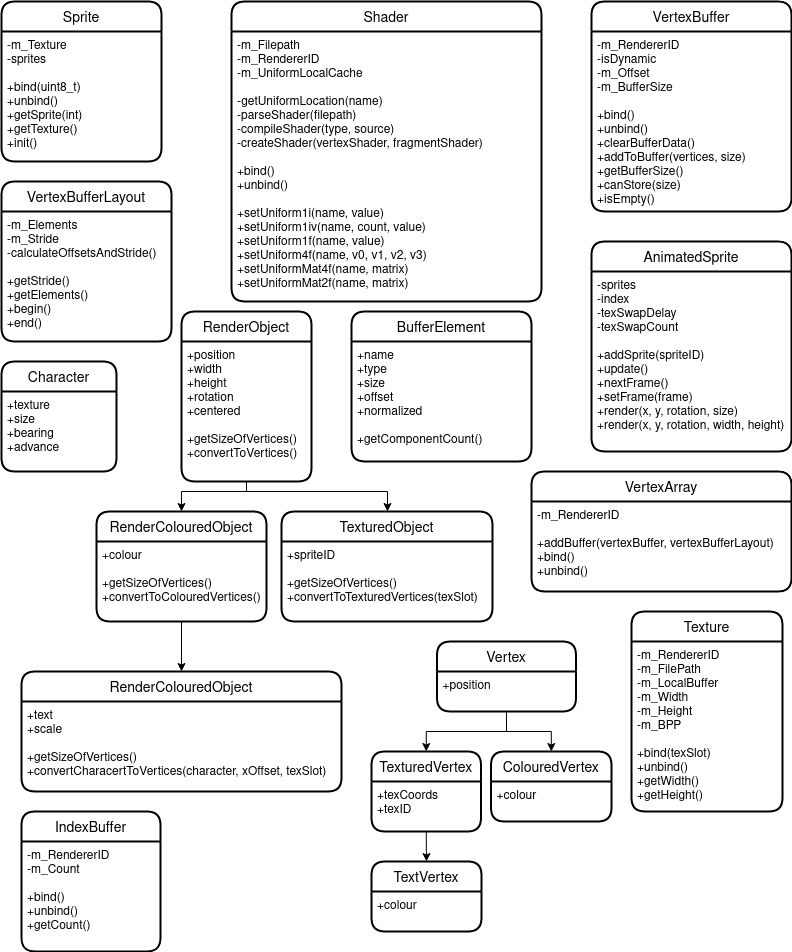
\includegraphics[scale=0.5]{img/Classes/Rendering Utils.png}}
        \caption{Classes involved in rendering}
        \label{fig}
    \end{figure}
    Sprite
    \begin{center}
        Variables
        \begin{tabular}{ | m{0.45\textwidth} | m{0.45\textwidth} | }
            \hline
            \textbf{Variable Name} & \textbf{Description} \\
            \hline
            m\_Texture & Stores the texture for that sprite \\
            \hline
            sprites & Array that stores all the current sprites in the program \\
            \hline
        \end{tabular}
        Functions
        \begin{tabular}{ | m{0.15\textwidth} | m{0.35\textwidth}| m{0.4\textwidth} | }
            \hline
            \textbf{Function Name} & \textbf{Parameters} & \textbf{Description} \\
            \hline
            bind & Slot ID & Binds the texture at a given slot \\
            \hline
            unbind & & Unbinds a given its texture \\
            \hline
            getSprite & Sprite ID & returns a sprite in the list \\
            \hline
            getTexture & & Returns its texture \\
            \hline
            init & & Run at the start of the program to initialise all the sprites \\
            \hline
        \end{tabular}
    \end{center}
    Shader
    \begin{center}
        Variables
        \begin{tabular}{ | m{0.45\textwidth} | m{0.45\textwidth} | }
            \hline
            \textbf{Variable Name} & \textbf{Description} \\
            \hline
            m\_Filepath & Used for debugging - Stores the filepath of the shader \\
            \hline
            m\_RenderID & openGL ID used for interactions with the shader \\
            \hline
            m\_UniformLocalCache & Stores all the locations of the uniforms in the shader for quick access \\
            \hline
        \end{tabular}
        Functions
        \begin{tabular}{ | m{0.15\textwidth} | m{0.35\textwidth}| m{0.4\textwidth} | }
            \hline
            \textbf{Function Name} & \textbf{Parameters} & \textbf{Description} \\
            \hline
            getUniformLocation & name of the variable & returns the location of the variable in the shader \\
            \hline
            parseShader & filepath to the shader & returns vertex and buffer shader from the filepath \\
            \hline
            compileShader & type of shader and the source of the shader & compiles the shader and returns ID \\
            \hline
            createShader & vertex and fragment shader code & compiles and links the shader \\
            \hline
            bind & & Binds the shader \\
            \hline
            unbind & & Unbinds the shader \\
            \hline
            setUniform1i & name of the variable and the integer & Attaches the value to the uniform \\
            \hline
            setUniform1iv & name of the variable and how many is in the list, then pointer to first element & Attaches the value to the uniform \\
            \hline
            setUniform1f & name of the variable then the float & Attaches the value to the uniform \\
            \hline
            setUniform4f & name of the variable then the four floats & Attaches the value to the uniform \\
            \hline
            setUniformMat4f & name and then the matrix & Attaches the value to the uniform \\
            \hline
            setUniformMat2f & name and then the matrix & Attaches the value to the uniform \\
            \hline
        \end{tabular}
    \end{center}
    VertexBufferLayout
    \begin{center}
        Variables
        \begin{tabular}{ | m{0.45\textwidth} | m{0.45\textwidth} | }
            \hline
            \textbf{Variable Name} & \textbf{Description} \\
            \hline
            m\_Elements & Stores the elements of the layout \\
            \hline
            m\_Stride & Stores the length of how long each vertex is \\
            \hline
        \end{tabular}
        Functions
        \begin{tabular}{ | m{0.2\textwidth} | m{0.3\textwidth}| m{0.4\textwidth} | }
            \hline
            \textbf{Function Name} & \textbf{Parameters} & \textbf{Description} \\
            \hline
            calculateOffsetsAndStride & & Calculates all the offsets for the elements \\
            \hline
            getStride & & Returns the stride \\
            \hline
            getElements & & Returns the elements \\
            \hline
            begin & & Go between function for the vector m\_Elements \\
            \hline
            end & & Go between function for the vector m\_Elements \\
            \hline
        \end{tabular}
    \end{center}
    Character
    \begin{center}
        Variables
        \begin{tabular}{ | m{0.45\textwidth} | m{0.45\textwidth} | }
            \hline
            \textbf{Variable Name} & \textbf{Description} \\
            \hline
            texture & Stores the texture for the character \\
            \hline
            size & A vector that stores the width and height of the character \\
            \hline
            bearing & A vector that stores the position relative to the origin \\
            \hline
            advance & Stores the position of the next character relative to itself\\
            \hline
        \end{tabular}
    \end{center}
    BufferElement
    \begin{center}
        Variables
        \begin{tabular}{ | m{0.45\textwidth} | m{0.45\textwidth} | }
            \hline
            \textbf{Variable Name} & \textbf{Description} \\
            \hline
            name & Stores the name of the variable input \\
            \hline
            type & Stores the type of the variable \\
            \hline
            size & Stores the size of the variable \\
            \hline
            offset & Stores the offset of its start position \\
            \hline
            normalized & Stores whether it is normalized \\
            \hline
        \end{tabular}
        Functions
        \begin{tabular}{ | m{0.15\textwidth} | m{0.35\textwidth}| m{0.4\textwidth} | }
            \hline
            \textbf{Function Name} & \textbf{Parameters} & \textbf{Description} \\
            \hline
            getCompoundCount & & Returns the count of elements in each type \\
            \hline
        \end{tabular}
    \end{center}
    VertexBuffer
    \begin{center}
        Variables
        \begin{tabular}{ | m{0.45\textwidth} | m{0.45\textwidth} | }
            \hline
            \textbf{Variable Name} & \textbf{Description} \\
            \hline
            m\_RendererID & Stores the ID of the buffer \\
            \hline
            m\_Offset & Stores the current offset of the buffer of inputting elements \\
            \hline
            m\_BufferSize & Stores the buffer size \\
            \hline
        \end{tabular}
        Functions
        \begin{tabular}{ | m{0.15\textwidth} | m{0.35\textwidth}| m{0.4\textwidth} | }
            \hline
            \textbf{Function Name} & \textbf{Parameters} & \textbf{Description} \\
            \hline
            bind & & Binds the buffer \\
            \hline
            unbind & & Unbinds the buffer \\
            \hline
            clearBufferData & & Clears all the data on the buffer \\
            \hline
            addToBuffer & pointer to the vertices and the size of the vertices & Adds data to the buffer \\
            \hline
            getBufferSize & & Returns the buffer size \\
            \hline
            canStore & Size of the data & Checks to see if it can store that data size \\
            \hline
            isEmpty & & Returns if the buffer is empty \\
            \hline
        \end{tabular}
    \end{center}
    AnimatedSprite
    \begin{center}
        Variables
        \begin{tabular}{ | m{0.45\textwidth} | m{0.45\textwidth} | }
            \hline
            \textbf{Variable Name} & \textbf{Description} \\
            \hline
            sprites & Stores all the sprite IDs \\
            \hline
            index & Stores the current index of the sprite it is on \\
            \hline
            texSwapDelay & Stores the delay between the animations \\
            \hline
            texSwapCount & Stores the counter for the update cycles between the increasing of the index \\
            \hline
        \end{tabular}
        Functions
        \begin{tabular}{ | m{0.15\textwidth} | m{0.35\textwidth}| m{0.4\textwidth} | }
            \hline
            \textbf{Function Name} & \textbf{Parameters} & \textbf{Description} \\
            \hline
            addSprite & sprite ID & Adds the sprite onto the animation \\
            \hline
            update & & Increases the count and goes to next sprite if needed \\
            \hline
            nextFrame & & Increases index by one \\
            \hline
            setFrame & frame index & Sets the frame to the input \\
            \hline
            render & Coords and rotation and either width and height or size & Renders the current sprite active \\
            \hline
        \end{tabular}
    \end{center}
    VertexArray
    \begin{center}
        Variables
        \begin{tabular}{ | m{0.45\textwidth} | m{0.45\textwidth} | }
            \hline
            \textbf{Variable Name} & \textbf{Description} \\
            \hline
            m\_RenderID & Stores the openGL ID \\
            \hline
        \end{tabular}
        Functions
        \begin{tabular}{ | m{0.15\textwidth} | m{0.35\textwidth}| m{0.4\textwidth} | }
            \hline
            \textbf{Function Name} & \textbf{Parameters} & \textbf{Description} \\
            \hline
            addBuffer & VertexBuffer to add and a layout to apply & Binds the vertex buffer to the vertex array and applies a layout to it \\
            \hline
            bind & & Binds the vertex array \\
            \hline
            unbind & & Unbinds the vertex array \\
            \hline
        \end{tabular}
    \end{center}
    Texture
    \begin{center}
        Variables
        \begin{tabular}{ | m{0.45\textwidth} | m{0.45\textwidth} | }
            \hline
            \textbf{Variable Name} & \textbf{Description} \\
            \hline
            m\_RenderID & Stores openGL ID for the texture \\
            \hline
            m\_FilePath & For debugging purposes stores the filepath of the texture \\
            \hline
            m\_LocalBuffer & Stores the pointer referring to its local buffer where the image is stored \\
            \hline
            m\_Width & Stores the width of the image \\
            \hline
            m\_Height & Stores the height of the image \\
            \hline
            m\_BPP & Stores the bytes per pixel \\
            \hline
            bufferStorage & Stores what textures are bound to what slot \\
            \hline
        \end{tabular}
        Functions
        \begin{tabular}{ | m{0.15\textwidth} | m{0.35\textwidth}| m{0.4\textwidth} | }
            \hline
            \textbf{Function Name} & \textbf{Parameters} & \textbf{Description} \\
            \hline
            bind & Slot to bind to & Binds image to given slot \\
            \hline
            unbind & & Unbinds the texture \\
            \hline
            getWidth & & Returns the width of the image \\
            \hline
            getHeight & & Returns the height of the image \\
            \hline
            getTextureInBuffer & texture slot & Returns the texture bound at that slot  \\
            \hline
            getBoundSlot & Texture & Returns the slot that the texture is bound to \\
            \hline
            clearBufferSlots & & Clears all the textures bound \\
            \hline
        \end{tabular}
    \end{center}
    IndexBuffer
    \begin{center}
        Variables
        \begin{tabular}{ | m{0.45\textwidth} | m{0.45\textwidth} | }
            \hline
            \textbf{Variable Name} & \textbf{Description} \\
            \hline
            m\_RenderID & Stores the openGL ID \\
            \hline
            m\_Count & Stores the amount of squares it can deal with \\
            \hline
        \end{tabular}
        Functions
        \begin{tabular}{ | m{0.15\textwidth} | m{0.35\textwidth}| m{0.4\textwidth} | }
            \hline
            \textbf{Function Name} & \textbf{Parameters} & \textbf{Description} \\
            \hline
            bind & & Binds the index buffer \\
            \hline
            unbind & & Unbinds the index buffer \\
            \hline
            getCount & & Returns count \\
            \hline
        \end{tabular}
    \end{center}
    RenderObject
    \begin{center}
        Variables
        \begin{tabular}{ | m{0.45\textwidth} | m{0.45\textwidth} | }
            \hline
            \textbf{Variable Name} & \textbf{Description} \\
            \hline
            position & Stores the position of the object \\
            \hline
            width & Stores the width of the object \\
            \hline
            height & Stores the height of the object \\
            \hline
            rotation & Stores the rotation of the object \\
            \hline
            centered & Stores whether the points are centered or not \\
            \hline
        \end{tabular}
        Functions
        \begin{tabular}{ | m{0.15\textwidth} | m{0.35\textwidth}| m{0.4\textwidth} | }
            \hline
            \textbf{Function Name} & \textbf{Parameters} & \textbf{Description} \\
            \hline
            getSizeOfVertices & & Returns the size of the vertices that is intended \\
            \hline
            convertToVertices & & Returns the object however in a array of 4 vertices \\
            \hline
        \end{tabular}
    \end{center}
    TexturedObject
    \begin{center}
        Variables
        \begin{tabular}{ | m{0.45\textwidth} | m{0.45\textwidth} | }
            \hline
            \textbf{Variable Name} & \textbf{Description} \\
            \hline
            spriteID & Stores the sprite id of the object \\
            \hline
        \end{tabular}
        Functions
        \begin{tabular}{ | m{0.2\textwidth} | m{0.3\textwidth}| m{0.4\textwidth} | }
            \hline
            \textbf{Function Name} & \textbf{Parameters} & \textbf{Description} \\
            \hline
            convertToTexturedVertices & texSlot of the sprite & returns textured vertices representation of the object \\
            \hline
        \end{tabular}
    \end{center}
    ColouredObject
    \begin{center}
        Variables
        \begin{tabular}{ | m{0.45\textwidth} | m{0.45\textwidth} | }
            \hline
            \textbf{Variable Name} & \textbf{Description} \\
            \hline
            colour & Stores a vec4 which represents the colour of the object \\
            \hline
        \end{tabular}
        Functions
        \begin{tabular}{ | m{0.2\textwidth} | m{0.3\textwidth}| m{0.4\textwidth} | }
            \hline
            \textbf{Function Name} & \textbf{Parameters} & \textbf{Description} \\
            \hline
            convertToColouredVertices & & Converts the object to coloured vertices \\
            \hline
        \end{tabular}
    \end{center}
    RenderTextObject
    \begin{center}
        Variables
        \begin{tabular}{ | m{0.45\textwidth} | m{0.45\textwidth} | }
            \hline
            \textbf{Variable Name} & \textbf{Description} \\
            \hline
            text & Stores the text of the object \\
            \hline
            scale & Stores the scale of the text \\
            \hline
        \end{tabular}
        Functions
        \begin{tabular}{ | m{0.25\textwidth} | m{0.25\textwidth}| m{0.4\textwidth} | }
            \hline
            \textbf{Function Name} & \textbf{Parameters} & \textbf{Description} \\
            \hline
            convertCharacterToVertices & character offset of the text position and the texture slot storing the character's texture & Converts the object into TextVertexes \\
            \hline
        \end{tabular}
    \end{center}
    Vertex
    \begin{center}
        Variables
        \begin{tabular}{ | m{0.45\textwidth} | m{0.45\textwidth} | }
            \hline
            \textbf{Variable Name} & \textbf{Description} \\
            \hline
            position & Stores the position of the vertex \\
            \hline
        \end{tabular}
    \end{center}
    ColouredVertex
    \begin{center}
        Variables
        \begin{tabular}{ | m{0.45\textwidth} | m{0.45\textwidth} | }
            \hline
            \textbf{Variable Name} & \textbf{Description} \\
            \hline
            colour & Stores the colour of the vertex \\
            \hline
        \end{tabular}
    \end{center}
    TexturedVertex
    \begin{center}
        Variables
        \begin{tabular}{ | m{0.45\textwidth} | m{0.45\textwidth} | }
            \hline
            \textbf{Variable Name} & \textbf{Description} \\
            \hline
            texCoords & Stores the position on the texture this vertex represents \\
            \hline
            texID & Stores the texture ID / slot of the texture it represents \\
            \hline
        \end{tabular}
    \end{center}
    TextVertex
    \begin{center}
        Variables
        \begin{tabular}{ | m{0.45\textwidth} | m{0.45\textwidth} | }
            \hline
            \textbf{Variable Name} & \textbf{Description} \\
            \hline
            colour & Stores the colour of the text \\
            \hline
        \end{tabular}
    \end{center}
\end{document}